\subsection{Separating Readout Fitting from Encoder Regularization}\label{app:protected_audit}

The learned-head arm changes both the reader and its features. To separate
these effects, we fixed a retrospective control before computing any new fits.
It uses every saved confirmation encoder from Appendix~\ref{app:protected_head}:
detached (D), unconstrained joint (J), and jointly protected (P), with ten seeds
per corpus. The original outcomes were already known. These controls therefore
do not constitute a new independent confirmation, and they leave the original
HAR $9/10$ and SNR $0/10$ decisions unchanged. Seeds $300$--$309$ are held out
from this experiment's development seeds, but were used in earlier studies.
The released plans and hashes record the protocols; their combined plan/result
commits do not establish an independent registration timestamp.

For each saved encoder, we fit an affine reader to the healthy teacher logits
on all fitting inputs, without labels. We center the targets, standardize the
features using fitting-set statistics, and solve either ordinary least squares
(OLS) or ridge regression with coefficient $10^{-3}$ and an unpenalized
intercept. OLS uses float64 SVD and tolerance
$\max(n,m)\,\epsilon\,s_{\max}$; feature standard deviations are floored at
$10^{-6}$. Both fits were fixed in the control plan, with no validation-based
choice. The encoder, current head and auxiliary head remain unchanged.

All six fitted readers and the original online head share a fresh uniform
$1{,}024$-input monitor per endpoint. The family contains $140$ consumers across
the two corpora and ten seeds, with total $\delta=0.05$ and the same five-point
budget. Table~\ref{tab:protected_audit} reports all fits, including the detached
controls; Figure~\ref{fig:protected_audit} compares the joint and protected
features. These are new bounds for fixed saved candidates, rather than
replacements for the original study's bounds.

\begin{table}[htbp]
\centering
\caption{Fixed retrospective teacher-head fits on saved encoders. All fits use training features and healthy logits without labels. D/J/P denote detached, unconstrained joint, and jointly protected encoders. Certificates use the same fresh monitor and 140-consumer family for every row; original 9/10 and 0/10 decisions remain unchanged. Means over ten saved seeds per corpus.}
\label{tab:protected_audit}
\footnotesize
\begin{tabular}{llrrr}
\toprule
Corpus & donor / legacy reader & accuracy & changed & certified \\
\midrule
HAR & D / ols & 0.911 & $0.97\%$ & $10/10$ \\
HAR & D / ridge & 0.911 & $1.15\%$ & $10/10$ \\
HAR & J / ols & 0.915 & $3.35\%$ & $1/10$ \\
HAR & J / ridge & 0.916 & $3.56\%$ & $0/10$ \\
HAR & P / ols & 0.914 & $1.44\%$ & $10/10$ \\
HAR & P / ridge & 0.914 & $1.50\%$ & $9/10$ \\
HAR & P / online & 0.915 & $1.77\%$ & $9/10$ \\
\midrule
SNR & D / ols & 0.269 & $38.58\%$ & $0/10$ \\
SNR & D / ridge & 0.273 & $39.80\%$ & $0/10$ \\
SNR & J / ols & 0.272 & $41.49\%$ & $0/10$ \\
SNR & J / ridge & 0.275 & $42.61\%$ & $0/10$ \\
SNR & P / ols & 0.259 & $4.04\%$ & $0/10$ \\
SNR & P / ridge & 0.259 & $5.36\%$ & $0/10$ \\
SNR & P / online & 0.259 & $5.00\%$ & $0/10$ \\
\bottomrule
\end{tabular}
\end{table}


On HAR, fitting OLS to the protected encoder reduces mean disagreement from
$1.77\%$ to $1.44\%$ and certifies all ten saved seeds. Reconstruction MSE and
current-head accuracy are unchanged by construction. Applying the identical
fit to the unconstrained joint encoder leaves $3.35\%$ disagreement and
certifies one seed; ridge certifies none. Thus a head-only fit on unrestricted
features does not recover the result of joint distillation. Regularizing the
encoder contributes to this comparison. OLS and ridge both recover the detached
control in all ten seeds, providing a check that the fitting procedure can
recover an accessible legacy function. On SNR, protected-feature OLS lowers
mean disagreement to $4.04\%$, but no seed certifies, and the original primary
accuracy loss remains. These outcomes establish neither information erasure
nor the impossibility of a richer reader.

\begin{figure}[H]
\centering
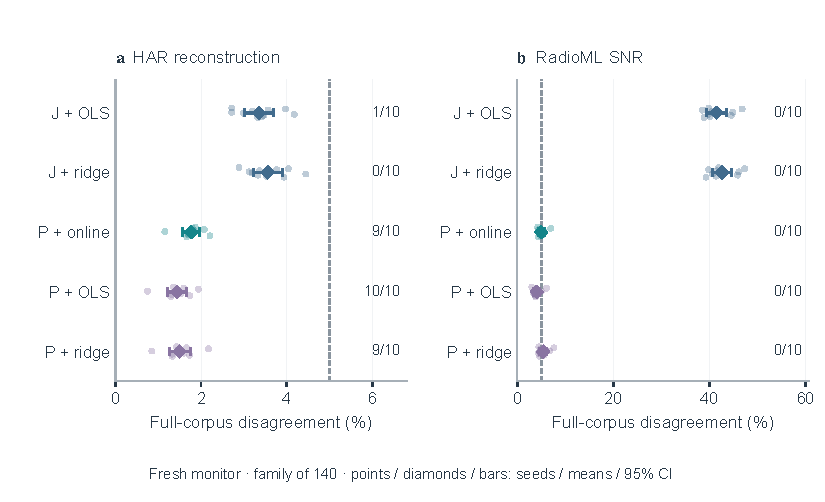
\includegraphics[width=\linewidth]{figures/fig_protected_audit.pdf}
\caption{A reader fit and encoder regularization have different effects. J and
P are the unconstrained joint and jointly protected encoders; online denotes
the head trained during continuation. Points show all saved seeds, diamonds
their means, and bars $95\%$ intervals across seeds. Counts are
certificates from the new $140$-consumer audit, while the horizontal coordinate
is full-corpus disagreement. The dashed line marks the $5\%$ budget; a mean
below it does not imply a certificate. All controls were specified after the
original outcomes were known.}
\label{fig:protected_audit}
\end{figure}

Independent numerical replay recovers all $60$ original legacy-consumer metric
sets exactly. A second process reloads the $120$ new affine readers and $20$
online heads without refitting, reproduces their metrics and bounds exactly,
and checks the convex fits' stationarity conditions; the largest residual is
$8.50\times10^{-10}$. Tensor states are retained locally; the supplementary
archive contains the numerical replay records and drivers.

The original timing closures used identical current-head operations for the
ordinary and protected paths, so they did not measure serving both outputs.
An isolated corrected benchmark returns current and legacy logits from a
single encoder call, using four CPU threads, five warm-ups and $51$
alternating repetitions per path. At batch $1{,}024$, the online protected
head costs $1.054\times$ current-only inference on HAR and $1.076\times$ on
SNR. The float64 OLS head costs $1.181\times$ and $1.243\times$, respectively.
At batch one, the corresponding ratios are $1.100/1.143$ on HAR and
$1.103/1.156$ on SNR (online/OLS). Ratios average per-seed medians. Encoder
features and online heads use float32; the current-head diagnostic evaluates
logits in float64, and the OLS reader is stored in float64. These measurements
establish the cost for these implementations, including both requested
outputs; parameter counts alone do not determine serving cost.
